% !TEX encoding = UTF-8
% !TEX TS-program = pdflatex
% !TEX root = ../tesi.tex
% !TEX spellcheck = it-IT

%**************************************************************
\chapter{Conclusioni}
\label{cap:conclusioni}
%**************************************************************
Al di là del formalismo informatico, lo scopo principale di questo progetto era indagare sul possibile uso della tecnologia \emph{Tango} nel campo ispettivo come effettivo supporto allo studio di beni materiali. Il prototipo realizzato sembra confermare che cioè è possibile.\\
I risultati ottenuti sono stati piuttosto soddisfacenti e con qualche raffinamento appare possibile inserire l'applicazione in un contesto produttivo.

\section{Prove pratiche}
Il prototipo prodotto è stato testato in numerosi ambienti e su diversi oggetti. Nella quasi totalità dei casi i risultati sono stati più che sufficienti per quanto riguarda la qualità del \emph{Point Cloud} ricostruito.\\
Per quanto riguarda invece il calcolo del volume i risultati non sono ancora totalmente sufficienti: il volume ottenuto è sempre dello stesso ordine di grandezza del volume reale, ma spesso è affetto da un errore relativo tra il 30 ed il 50\% ed un errore del genere non è affatto tollerabile. Tale divario però è facilmente appianabile migliorando la qualità delle elaborazioni dei \emph{Point Cloud} e delle \emph{mesh} lato \emph{Server}.

\section{Sviluppi futuri}
Il progetto è nato molto recentemente, dopo circa due mesi di sviluppo è stato prodotto un prototipo soddisfacente. Molti dei problemi riscontrati durante il percorso di \emph{stage} sono stati risolti, grazie ai prototipi e alle prove pratiche sono state molteplici anche le idee per rendere l'applicazione ancora più completa. Riporto qui solo alcune di queste.

\subsection{ICP su tablet}
Uno più gravi problemi delle ricostruzioni 3D effettuate tramite sovrapposizione di \emph{Point Cloud} è il \emph{ghosting}. Si tratta dello sdoppiamento di alcune "facce" dell'oggetto ricostruito.\\
\begin{figure}[!h] 
    \centering 
    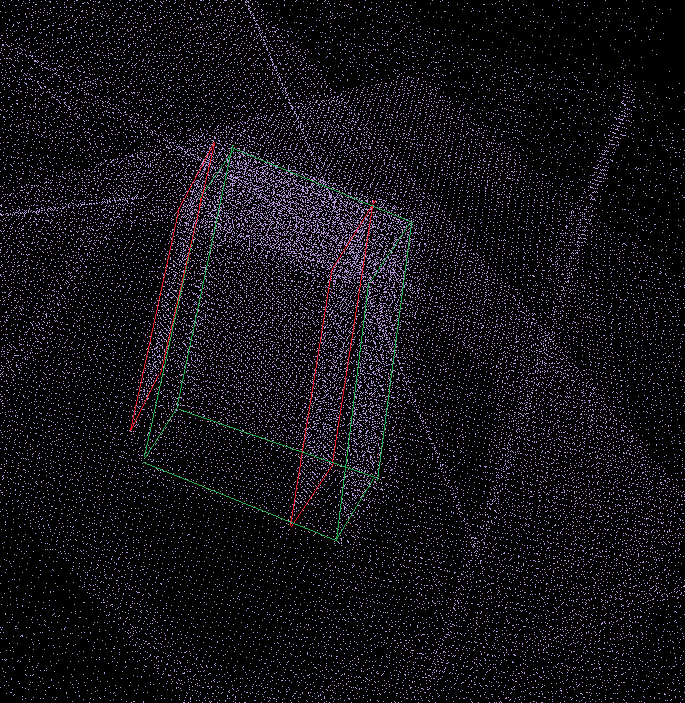
\includegraphics[width=0.9\columnwidth]{pointClouds/ghosting.png} 
    \caption{Point Cloud che presenta problemi di \emph{ghosting} di una scatola rettangolare}
    \label{figure:pcloud_ghosting}
\end{figure}
Nell'esempio in figura \ref{figure:pcloud_ghosting} sono stati evidenziati in verde gli spigoli corretti di una scatola rettangolare, mentre con colore rosso quelli dovuti al \emph{ghosting}; si può chiaramente notare che le facce laterali appaiono sdoppiate e ciò può portare a significativi errori nella ricostruzione dell'oggetto e soprattutto nel calcolo del volume.\\
Questo fenomeno è dovuto ad errori di stima nella posizione del dispositivo, e per quanto si cerchi di ridurli essi rimarranno sempre. Si tratta di un altro limite fisico dei dispositivi \emph{Tango}, che in questo caso è aggirabile.\\
\emph{ICP} o \emph{Iterative Closest Point} è un algoritmo che cerca di minimizzare le differenze tra due nuvole di punti. Applicando \emph{ICP} su due \emph{Point Cloud} che non si sovrappongono perfettamente permetterebbe di ottenere una matrice di trasformazione da applicare ad uno dei due per farlo combaciare all'altro. L'algoritmo in questione ha molte implementazioni in \emph{C++}, tra cui una presente proprio all'interno della libreria \emph{PCD} utilizzata lato \emph{Server}. Questo fatto ha dato modo di testare la sua effettiva efficacia.\\
Il problema è che spedire ogni singola ripresa al \emph{Server} ed aspettare una risposta sembra una strada non percorribile: per una rilevazione intera servono più di 20 riprese, senza connessione internet il servizio non sarebbe disponibile etc.\\
Per questo un possibile sviluppo futuro potrebbe essere quello di implementare \emph{ICP} lato \emph{tablet}. Ci sarebbe due vie percorribili: importare una delle tante implementazioni in \emph{C++} ed accedervi dal codice \emph{Java} mediate \emph{JNI} oppure implementare da capo l'algoritmo nativamente in \emph{Java}. Entrambe le ipotesi vanno attentamente valutate tenendo conto anche della potenza di calcolo e del consumo di batteria del dispositivo.

\subsection{Integrazione C++/Jni lato tablet}
\emph{Google} fornisce oltre a delle ricche librerie \emph{Java} anche delle \emph{API} in linguaggio \emph{C/C++}. Alcune funzioni esposte da queste ultime non sono presenti in quelle \emph{Java} oppure sono molto più efficienti. Sarebbe quindi necessario, negli sviluppi futuri, predisporre una interfaccia \emph{Jni} in maniera da integrare codice \emph{Java} e \emph{C++} all'interno della stessa applicazione.\\
Tutto il progetto ne gioverebbe, specialmente per quanto riguarda le performance; inoltre si potrebbe pensare di importare parti della libreria \emph{PCD} in maniera da automatizzare alcuni processi.

\subsection{Texture dei punti}
Il prodotto fornisce delle buone ricostruzioni 3D per quanto riguarda la forma e le dimensioni dell'oggetto; ai fini ispettivi, di fatto, non c'è bisogno d'altro. Ciononostante le ricostruzioni visualizzate sia su \emph{tablet} che su \emph{computer} essendo formate da soli punti sono spesso di difficile comprensione da parte dell'utenza. Per rispondere a queste esigenza potrebbe essere opportuno pensare ad aggiungere ad ogni singolo punto una opportuna texture in maniera da rendere più immediato il riconoscimento dell'oggetto da parte dell'utente.\\
Questo sviluppo darebbe un grosso valore aggiunto in quando migliora grandemente l'aspetto grafico del sistema e lo rende quindi anche più vendibile.\\
Alcuni esempi di \emph{Point Cloud} \emph{texturizzati} sono già presenti in rete sotto licenza \emph{Open Source}, quindi è possibile pensare al riuso degli stessi.

\subsection{Rimozione artefatti}
Un altro problema che affligge le ricostruzioni 3D effettuate da \emph{Samba} è il rumore causato da forti fonti di luce o superfici riflettenti.\\
In molte riprese infatti appaiono dei piani sospesi a mezz'aria che si sommano li uni agli altri rendendo qualche volta la ricostruzione praticamente inutilizzabile. Lato \emph{Server} essi sono spesso eliminabili dalla libreria \emph{PCD}, ma lato \emph{tablet} rendono la visualizzazione dei \emph{Point Cloud} ricostruito ancora più caotica e difficilmente usabile.\\
Un possibile sviluppo è quindi quello di usare le caratteristiche stesse di questi artefatti (come essere isolati, sempre perfettamente planari etc) per filtrarli già durante la ripresa del singolo \emph{Point Cloud} lato \emph{tablet}. In figura \ref{figure:pcloud_artifacts} sono stati evidenziati in rosso alcuni degli artefatti.
\begin{figure}[H] 
    \centering 
    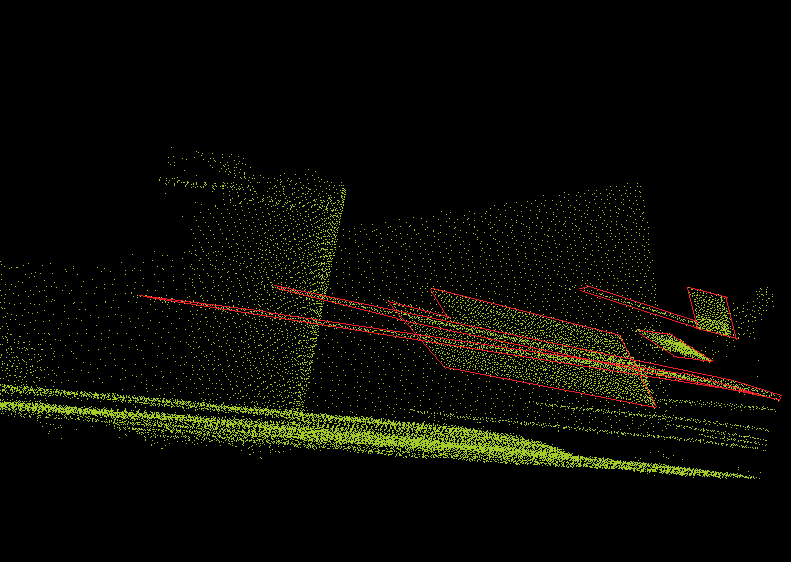
\includegraphics[width=0.9\columnwidth]{pointClouds/artefatti.png} 
    \caption{Point Cloud che presenta problemi di artefatti di un bidone conico, vista laterale}
    \label{figure:pcloud_artifacts}
\end{figure}

\subsection{Controllo di forma}
Oltre alla creazione del modello 3D e del calcolo del volume potrebbe rivelarsi molto utile per gli ispettori avere uno strumento automatico per confrontare la forma dell'oggetto ispezionato con un modello "perfetto" del bene stesso. Ad esempio potrebbe essere usato per confrontare componenti meccaniche con i loro modelli \emph{CAD} al fine di individuare eventuali deformazioni subite durante il trasporto.

\subsection{Integrazione con l'applicazione Vic}
L'azienda fornisce ai suoi dipendenti ispettori una applicazione che permette di automatizzare diverse mansioni. Tra le varie funzioni che mette a disposizione c'è quella di avviare una nuova ispezione o \emph{job} permettendo all'utente di compilare diversi \emph{form} per fornire così in tempo reale un rapporto dettagliato e standardizzato del lavoro svolto. In questo ambito una buona integrazione delle tecnologie \emph{Tango} potrebbe fornire molto valore aggiunto.


\subsection{Ricostruzione continua}
Le ricostruzioni di \emph{Samba} vengono effettuate "foto per foto", ovvero l'utente deve osservare l'oggetto da diverse angolazioni ed effettuare delle rilevazioni proprio come se si scattassero molte foto.\\
Un ottimo sviluppo sarebbe fare in modo che queste rilevazioni fossero effettuate in maniera automatica e continua, ciò darebbe molti vantaggi al sistema:
\begin{itemize}
	\item Ci sarebbero molti più dati, quindi la rilevazione sarebbe di maggiore qualità.
	\item L'applicazione sarebbe più vicina ai bisogni dell'utente.
	\item Si genererebbero molti \emph{Point Cloud} quasi uguali sovrapposti offrendo la possibilità di eliminare parte del rumore con metodi statistici (è improbabile che due scatti successivi dello stesso oggetto senza muovere il tablet siano affetti dagli stessi artefatti).
\end{itemize}
Apre però anche a nuovi problemi:
\begin{itemize}
	\item Maggiore carico di informazioni che deve essere gestito ed ottimizzato.
	\item Maggior consumo della batteria.
	\item Necessità di euristiche per determinare quale sia un \emph{Point Cloud} buono: l'utente non può più visionarli e scartare quelli affetti da errore.
\end{itemize}


\section{Problemi ancora irrisolti}

\subsection{Surriscaldamento e consumo della batteria}
Il prototipo prodotto ha un consumo della batteria piuttosto elevato ed a volte porta al surriscaldamento del dispositivo.
Ciò secondo una prima analisi è dovuto ai seguenti fattori:
\begin{itemize}
	\item Utilizzo combinato dei quattro sensori principali del \emph{device}: fotocamera a colori, fotocamera \emph{Fish-eye}\footnote{Fotocamera \emph{Fish-eye}: un obbiettivo grandangolare che abbraccia un angolo di campo di circa 180 gradi, in particolare quello in dotazione nel dispositivo usato è in bianco e nero.}, sensore \emph{IR} ed accelerometro/giroscopio. Questi sensori sono tutti necessari per il \emph{Motion Tracking} e la cattura dei \emph{Point Cloud}.
	\item Grande mole di dati da elaborare: un singolo \emph{Point Cloud} può contare anche 90 000 punti, essi devono essere elaborati e renderizzati in tempo reale.	
	\item Necessità di pesanti elaborazioni parallele: per permettere all'utente una interfaccia fluida e non rallentare i calcoli è necessario usare molti processi paralleli. Ogni scatto registrato è elaborato su di un proprio \emph{Thread} ed è presente un servizio che ottimizza ad intervalli regolari la ricostruzione corrente (indispensabile per tenere sotto controllo la complessità delle strutture dati).
	\item \emph{Rendering real-time}: come discusso in sezione \ref{cap:frame_preview} è un fondamentale requisito di usabilità avere una preview dei dati catturati dal \emph{depth sensor}. Ciò implica l'utilizzo di un \emph{render 3D} \emph{OpenGL} che richiede una grande quantità di risorse.
	\item Connessione dati: la necessità di un \emph{backend Server} comporta l'utilizzo della connessione internet. Inoltre dato il tipo di utilizzo per cui è stata ideata l'applicazione userà spesso la connessione \emph{mobile} per inviare i dati.
\end{itemize}
Risolvere queste criticità era oltre gli obiettivi dello \emph{stage}, ma è comunque stato stilato un documento contenente alcune contromisure che potranno essere usate per mitigarne gli effetti:
\begin{itemize}
	\item Effettuare le operazioni più dispendiose usando le librerie native in \emph{C} ed integrarne i risultati mediante una interfaccia \emph{Jni}.
	\item Una volta migrate le operazioni di elaborazione dei punti da \emph{Java} a \emph{C} si dovrebbero avere un sensibile incremento nelle prestazioni che permetterebbe di limitare l'elaborazione a solo due processi: uno per gestire la trasformazione dei punti (rotazione, traslazione, sovrapposizione) ed uno per le operazioni di ottimizzazione (\emph{voxeling}, rimozione rumore, rimozione ridondanze).
	\item Gestire la priorità del servizio di ottimizzazione: è trasparente all'utente e non deve necessariamente essere performante. Quindi esso può avere una minore priorità nell'utilizzo della \emph{CPU} cercando di ridurre i \emph{burst} di dati.
	\item Il \emph{render} non ha lo scopo di rappresentare tutti i punti salvati, ma di fornire all'utente una idea di quello che "vede" il sensore di profondità. Si può pensare quindi di approssimare parti della nuvola di punti a figure geometriche semplici, ad esempio il pavimento può essere approssimato ad un piano. Ciò ridurrebbe il carico di lavoro per processore e scheda grafica.
\end{itemize}
Comunque va tenuto a mente che il dispositivo è un \emph{HardWare} sperimentale che non è pensato per utilizzo su larga scala ma solo per lo sviluppo: comportamento instabile del dispositivo usando alcuni tipi di applicazioni è largamente documentato all'interno della comunità. xxxx (documentare)\\
Durante il tirocinio sono stati sperimentati questo genere di problemi anche con applicazioni rilasciate dalla \emph{Google} stessa. xxxx (documentare)

\subsection{Preview della fotocamera}
Le \emph{API} forniscono degli strumenti per automatizzare la \emph{preview} della fotocamera a colori. Essi tuttavia si sono rivelati estremamente pesanti come carico computazionale e se combinati al resto dell'applicazione prodotta possono portare a rallentamenti imprevisti.\\
Per questo si è scelto di ottenere questa anteprima tramite metodi di basso livello. Essi tuttavia richiedono uno sforzo ben maggiore e quelli applicati in \emph{Samba} vanno rivisti.\\
Un \emph{bug} noto è che alla ripresa della attività, qualche volta la \emph{preview} non viene attivata ed il riquadro a lei riservato rimane nero.


%**************************************************************
\section{Consuntivo finale}
Il periodo di \emph{stage} ha avuto avvio il 13 Giugno 2016 ed è terminato il 16 Agosto 2016 invece che il 5 Agosto. Lo slittamento della data di fine è dovuto ad impegni universitari dello studente ed a un breve periodo di chiusura estiva dell'azienda. Il tirocinio ha avuto una durata totale di 320 ore.\\
In tabella \ref{tab:preventivo-consuntivo} sono riportate le ore preventivate per ogni attività ed esse sono confrontate con le ore effettivamente impiegate.
\begin{table}[H]
	\begin{center}
	  \begin{tabular}{| l | c | c | c | c |}
	    \hline
	    \textbf{Attività} & \textbf{Preventivo} & \textbf{Consuntivo} & \textbf{Diff} & \textbf{Diff \%} \\ \hline
	    Studio preliminare & 20 & 24 & +4 & +20\%\\
	    \hline
	    Ideazione modello di soluzione & 20 & 16 & -4 & -20\%\\
	    \hline
	    Studio di fattibilità/analisi dei rischi & 20 & 32 & +12 & +60\%\\
	    \hline
	    Analisi dei requisiti & 20 & 12 & -8 & -40\%\\
	    \hline
	    Prototipi preliminari & 40 & 86 & +46 & +115\%\\
	    \hline
	    Progettazione & 40 & 30 & -10 & -25\%\\
	    \hline
	    Codifica & 120 & 80 & -40 & -33,3\%\\
	    \hline
	    Verifica e validazione & 30 & 25 & -5 & -16,6\%\\
	    \hline
	    Prove pratiche & 10 & 15 & +5 & +50\%\\
	    \hline
	    Totale & 320 & 320 & +0 & +0\%\\
	    \hline
	  \end{tabular}
	\end{center}
	\caption{Distribuzione ore preventivo e consuntivo}\label{tab:preventivo-consuntivo}
\end{table}
Le ore totali sono state rispettate e non hanno avuto variazioni.\\
La loro ripartizione interna, invece, ha subito grosse variazioni a causa di sovrastime e sottostime commesse durante la fase di pianificazione.\\
Le attività che hanno subito variazioni più importanti sono state codifica e sviluppo dei prototipi preliminari. Questi ultimi hanno richiesto più del doppio del tempo preventivato a causa della difficoltà del compito richiesto, ma soprattutto perché lo studente ha intrapreso una strada sbagliata che ha portato ad un prototipo non funzionante e che è stato interamente scartato. Si può notare però che la maggiore attenzione riposta nei prototipi preliminari ha fatto risparmiare diverse ore alla codifica: infatti molto del codice presente nei primi prototipi è stato riusato senza cambiamenti, o con modeste modifiche.\\
Anche lo studio di fattibilità ha richiesto più tempo del previsto in quanto si è rivelato necessario cercare e provare molte applicazioni, alcune delle quali non manutenute o non aggiornate.\\
In figura \ref{gantt:pianificaiozne} vengono riportati i diagrammi di \emph{Gantt} dove è possibile confrontare la pianificazione preventivata e quella effettiva.

\begin{figure}[H] 
    \centering 
    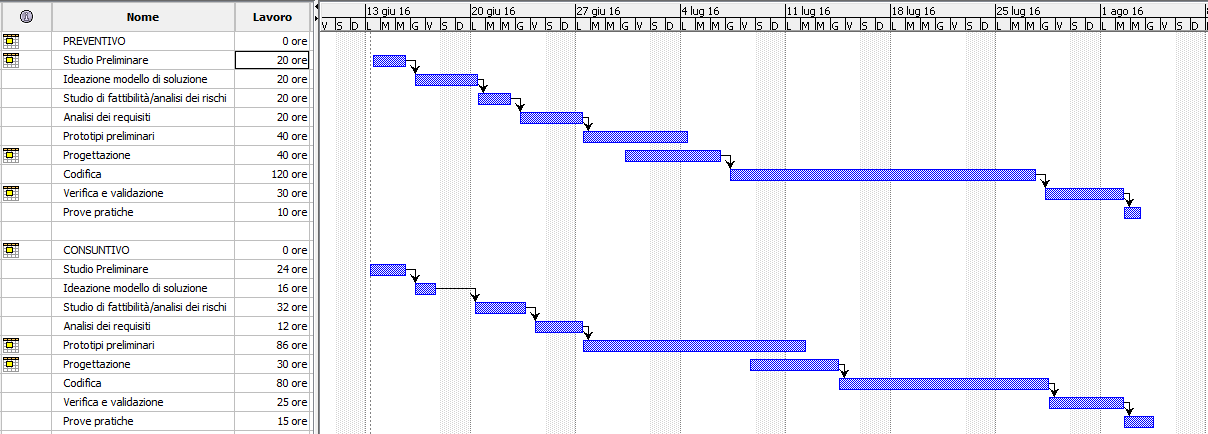
\includegraphics[width=1.0\columnwidth]{varie/ganttConsuntivo.png} 
    \caption{Gantt della pianificazione preventiva e consuntiva}
    \label{gantt:pianificaiozne}
\end{figure}

%**************************************************************
\section{Raggiungimento degli obiettivi}
\subsection{Obiettivi generali}
Gli obiettivi generali riportati nel piano di lavoro erano i seguenti:
\begin{itemize}
	\item Obbligatori
	\begin{itemize}
		\item \underline{\textit{ob01}}: studio delle soluzioni esistenti;
		\item \underline{\textit{ob02}}: ideazione di una soluzione per il riconoscimento di un oggetto;
		\item \underline{\textit{ob03}}: implementazione prototipo in grado di riconoscere un oggetto;
		\item \underline{\textit{ob04}}: calcolo del volume dell'oggetto (approssimato);
		\item \underline{\textit{ob05}}: implementazione app come indicato nella sezione \emph{Struttura applicazione} del documento \emph{Relazione app per Project Tango} fornito dall'azienda;
	\end{itemize}
	
	\item Desiderabili 
	\begin{itemize}
		\item \underline{\textit{de01}}: generare modello 3D in un formato portabile (obj, ply, vtk);
		\item \underline{\textit{de02}}: stima della precisione con cui viene ricostruito un oggetto;
		\item \underline{\textit{de03}}: perfezionare calcolo del volume (cavità nell'oggetto, elimanazione dati di sfondo/rumore);
		\item \underline{\textit{de04}}: stima della precisione nel calcolo del volume;
	\end{itemize}
	
	\item Opzionali
	\begin{itemize}
		\item \underline{\textit{op01}}: ottimizzazione della comunicazione con il server nel caso risultasse necessaria.
	\end{itemize} 
\end{itemize}

I requisiti obbligatori sono stati tutti raggiunti.\\
Per quanto riguarda quelli desiderabili invece:
\begin{itemize}
	\item \underline{\textit{de01}}: È stato pienamente soddisfatto.
	\item \underline{\textit{de02}}: Sono stati forniti molti modelli grafici, da cui è possibile effettuare delle considerazioni sulla precisione con cui vengono ricostruiti gli oggetti.
	\item \underline{\textit{de03}}: Non soddisfatto.
	\item \underline{\textit{de04}}: Sono stati condotti degli studi, ma si è ritenuto che l'applicazione fosse ad uno stato ancora troppo poco avanzato perché la statistica avesse senso.
\end{itemize}
Il requisito opzionale \underline{\textit{op01}} non è stato raggiunto.

\subsection{Requisiti}
Dagli obiettivi posti nel piano di lavoro sono stati ricavati i requisiti esposti nel capitolo \ref{cap:analisi-requisiti}. Seguono le tabelle di soddisfacimento di questi ultimi divisi per categorie.

\subsubsection{Requisiti funzionali}
\LTXtable{\textwidth}{tabelle/requisiti/soddisfacimento/funzionali.tex}
Segue una tabella riassuntiva di questa tipologia di requisiti.
\begin{table}[H]
	\begin{center}
	  \begin{tabular}{ l  c  c  c }
	    \hline
	    \textbf{Tipologia} & \textbf{Totali} & \textbf{Soddisfatti} & \textbf{Percentuale} \\ \hline
	    Obbligatori & 44 & 44 & 100\%\\ \hline
	    Desiderabili & 2 & 0 & 0\%\\
	    \hline
	  \end{tabular}
	\end{center}
	\caption{Tabella riassuntiva del soddisfacimento dei requisiti funzionali}
\end{table}

\subsubsection{Requisiti qualitativi}
\LTXtable{\textwidth}{tabelle/requisiti/soddisfacimento/qualitativi.tex}
Segue una tabella riassuntiva di questa tipologia di requisiti.
\begin{table}[H]
	\begin{center}
	  \begin{tabular}{ l  c  c  c }
	    \hline
	    \textbf{Tipologia} & \textbf{Totali} & \textbf{Soddisfatti} & \textbf{Percentuale} \\ \hline
	    Obbligatori & 3 & 3 & 100\%\\ \hline
	    Desiderabili & 1 & 1 & 100\%\\
	    \hline
	  \end{tabular}
	\end{center}
	\caption{Tabella riassuntiva del soddisfacimento dei requisiti qualitativi}
\end{table}

\subsubsection{Requisiti di vincolo}
\LTXtable{\textwidth}{tabelle/requisiti/soddisfacimento/vincolo.tex}
Segue una tabella riassuntiva di questa tipologia di requisiti.
\begin{table}[H]
	\begin{center}
	  \begin{tabular}{ l  c  c  c }
	    \hline
	    \textbf{Tipologia} & \textbf{Totali} & \textbf{Soddisfatti} & \textbf{Percentuale} \\ \hline
	    Obbligatori & 2 & 2 & 100\%\\
	    \hline
	  \end{tabular}
	\end{center}
\caption{Tabella riassuntiva del soddisfacimento dei requisiti di vincolo}
\end{table}	

\subsubsection{Requisiti prestazionali}
\LTXtable{\textwidth}{tabelle/requisiti/soddisfacimento/prestazionali.tex}
Segue una tabella riassuntiva di questa tipologia di requisiti.
\begin{table}[H]
	\begin{center}
	  \begin{tabular}{ l  c  c  c }
	    \hline
	    \textbf{Tipologia} & \textbf{Totali} & \textbf{Soddisfatti} & \textbf{Percentuale} \\ \hline
	    Obbligatori & 2 & 2 & 100\%\\ \hline
	    Desiderabili & 8 & 8 & 100\%\\
	    \hline
	  \end{tabular}
	\end{center}
\caption{Tabella riassuntiva del soddisfacimento dei requisiti prestazionali}
\end{table}	
Attenzione particolare è stata posta al requisito \emph{RDP-1.2}. Esso richiede che sia possibile effettuare almeno 5-6 catture al secondo. Studi sperimentali condotti in diversi ambienti confermano che le rilevazioni impiegano in media circa 220 millisecondi ad essere elaborato, quindi circa 4,5 riprese al secondo. È però possibile in ogni caso far effettuare un numero arbitrario di rilevazioni, che verranno elaborate su \emph{thread} paralleli, e anche se la loro elaborazione richiede più di un secondo è quindi possibile effettuare le 5-6 riprese a secondo richieste a patto di essere disposti ad aspettare qualche tempo per la loro elaborazione. Per questo il requisito è segnalato come parzialmente soddisfatto.


\subsubsection{Soddisfacimento requisiti}
Segue una tabella generale che riassume la copertura di tutti i requisiti.
\begin{table}[H]
	\begin{center}
	  \begin{tabular}{ l  c  c  c }
	    \hline
	    \textbf{Tipologia} & \textbf{Totali} & \textbf{Soddisfatti} & \textbf{Percentuale} \\ \hline
	    Obbligatori & 51 & 51 & 100\%\\ \hline
	    Desiderabili & 11 & 9 & 81,8\%\\
	    \hline
	  \end{tabular}
	\end{center}
\caption{Tabella riassuntiva del soddisfacimento di tutti i requisiti}
\end{table}	
%**************************************************************
\section{Conoscenze acquisite}
Dal punto di vista formativo l'attività di \emph{stage} è stata estremamente positiva. Ha arricchito il mio bagaglio personale di competenze professionali.\\

La richiesta di app \emph{mobile} è in continuo aumento. Per questo l'apprendimento della progettazione e sviluppo delle applicazioni mobili \emph{Android} è certamente una pietra miliare in campo \emph{IT} in questi anni.\\

L'approccio ad una tecnologia sperimentale ed ancora di nicchia come \emph{Tango Project} crea dei vantaggi in ambito occupazionale in quanto gli sviluppatori non sono molti. Inoltre il rilascio del primo \emph{smartphone} commerciale dotato dei sensori \emph{Tango} è stato annunciato da un noto marchio per settembre 2016; se dovesse prendere campo anche in ambito \emph{customer} ci sarebbe certamente una grande richiesta di sviluppatori con esperienza vista la scarsità di applicazioni dedicate a questo tipo di \emph{HardWare}. Altro aspetto positivo è stato l'inserimento all'interno della comunità degli sviluppatori \emph{Tango} sia su \emph{StackOverflow} che su \emph{Google plus}; lo studente ha avuto modo di confrontarsi con addetti \emph{Google} e con altri sviluppatori sia in ambito accademico/di ricerca che in ambito industriale.\\

In ambito aziendale si è usato \emph{Java} come linguaggio di programmazione ed \emph{Android Studio} come \emph{IDE}. La curva di apprendimento di questi strumenti è stata piuttosto rapida grazie all'esperienza già maturata in ambito accademico con \emph{Java} ed \emph{ItelliJ}, su cui è basato \emph{Android Studio}. Più complessa si è rivelata l'assimilazione e la comprensione del \emph{Framework Jni}, sia a causa della sua intrinseca compessità sia al fatto che \emph{Android Studio} lo supporta solo in \emph{release} sperimentale. Infatti in azienda è stato realizzato sono un piccolo prototipo che dimostra l'agibilità di questa via, ma poi la tecnologia \emph{Jni} è stata abbandonata in favore di uno sviluppo interamente in \emph{Java}. In ogni caso molte applicazioni \emph{mobile} specialmente in ambito grafico ne fanno uso, quindi ai fini del curriculum si è rivelata comunque un'esperienza fruttuosa.\\

In generale ritengo l'approccio a librerie grafiche sia \emph{mobile} che per \emph{PC} estremamente interessante ai fini della formazione personale.\\

L'apprendimento delle potenzialità della libreria \emph{PCL} e la gestione dei \emph{Point Cloud} è altrettanto importante, anche perché è uno dei pochi ambiti in cui l'Italia spicca in ambito di \emph{Computer} grafica.


%**************************************************************
%\section{Valutazione personale}







